\label{chap:jueces}

En esta sección se resolverán 2 problemas relacionados con \textit{string matching} usando el
algoritmo KMP y la función de error de la que se habló en el capítulo 4. Se resolverán los
problemas usando C++ y Haskell y se compararán ambas versiones.

Es un estándar que las especifiaciones del problema estén en inglés.

%% TODO: Explicar los constraints

\section{SPOJ}
SPOJ (Sphere Online Judge)
% https://wiki.haskell.org/SPOJ
% Tomar algo del competitive aquí

\section{Problemas}

\subsection{Encontrar el factor de repetición de una cadena}
Recordemos en el \hyperlink{repetition_factor}{capítulo 3 el problema 32.1}, es aquí cuando lo
bonito de la programación competitiva y resolver ejercicios teóricamente se juntan. Ése problema
es lo mismo a resolver el siguiente, y aún mejor, en un juez en línea que puede ``probar'' la
implementación considerando ciertas restricciones.

La especificación del problema dice lo siguiente: 

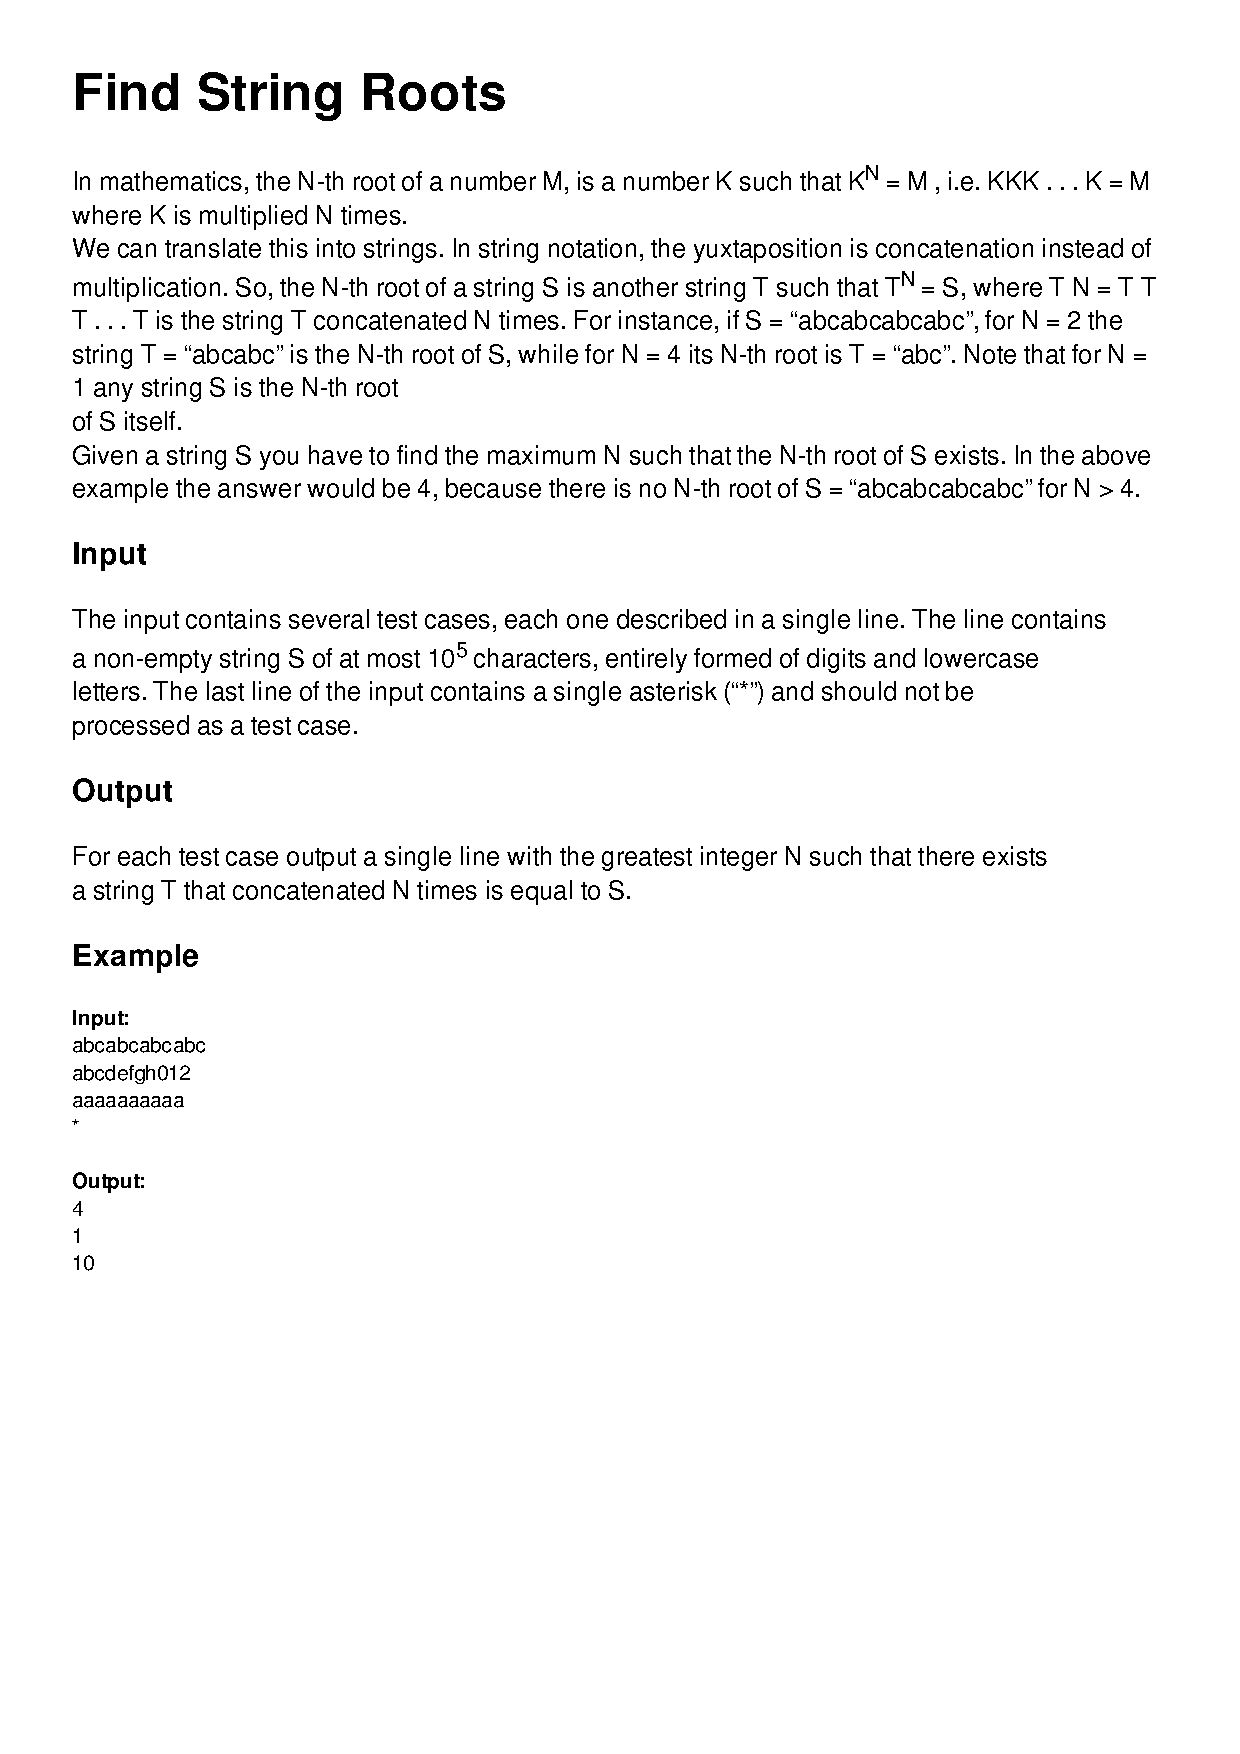
\includepdf[pages=-]{problemas/pdf/FINDSR.pdf}

Analisemos detenidamente la especificación del problema. 
\subsubsection{Análisis}
Como se había dicho previamente, ya se había atacado este problema así que se omitirá el análisis
y la complejidad.

\subsubsection{Entrada}
Una \textit{heurística} a seguir es que siempre que diga: \textit{``the input contains several test
cases, each line described in a single line''} es leer hasta el final de archivo (End Of File) cada
línea. Seguido de esto, dice que cada línea una cadena no vacía de a lo más $10^5$
caracteres\footnote{Hay lenguajes programación que no tienen implementadas cadenas, y que se debe
saber de antemano el tamaño, para así tener un arreglo de $n$ caracteres. Es aquí cuando es
importante saber el tamaño máximo de la entrada.} formada solamente de dígitos y letras en
minúsculas\footnote{También es sumamente importante saber si las cadenas del lenguaje que se usará
como son represntadas ya que podrían estar en ASCII o Unicode.}.
Finalmente dice que la última entrada contiene un solo asterisco \texttt{*} y que no debe ser
procesado como un caso más.

\subsubsection{Salida}
Para cada caso prueba \textit{(input)} se debe imprimir en la salida estándar una sola línea con un
número $n$ siendo ésta la raíz de la cadena, es decir, el número de veces que está concatenada la
cadena consigo misma.

\subsubsection{Ejemplos}
\begin{itemize}
\item Consideremos la entrada $x =$ \texttt{abcabcabcabc} y sobre ésta se construye la función
de error, 
\begin{table}[h]
\centering
\begin{tabular}{c|c|c|c|c|c|c|c|c|c|c|c|c|}
\cline{2-13}
$i$      & 1          & 2          & 3          & 4          & 5          & 6          & 7          & 8          & 9          & 10         & 11         & 12         \\ \hline
$P[i]$   & \texttt{a} & \texttt{b} & \texttt{c} & \texttt{a} & \texttt{b} & \texttt{c} & \texttt{a} & \texttt{b} & \texttt{c} & \texttt{a} & \texttt{b} & \texttt{c} \\ \hline
$\pi[i]$ & 0          & 0          & 0          & 1          & 2          & 3          & 4          & 5          & 6          & 7          & 8          & 9          \\ \cline{2-13} 
\end{tabular}
\end{table}

Siendo $\vert x \vert = 12$ y el último elemento de la función de error es $\pi[m] = 9$ y sea
$r = 12 - 9 = 3$. Se conluye que la raíz de la cadena es de longitud \textbf{3} y su factor de
repetición es $\rho(x) = \frac{12}{3} =$ \textbf{4}. Concluyendo así que
\texttt{(abc)}$^4 = $ \texttt{abcabcabcabc}.

\item Consideremos la entrada $x =$ \texttt{acbdefgh012} y sobre ésta se construye la función
de error, 
\begin{table}[h]
\centering
\begin{tabular}{c|c|c|c|c|c|c|c|c|c|c|c|}
\cline{2-12}
$i$      & 1          & 2          & 3          & 4          & 5          & 6          & 7          & 8          & 9          & 10         & 11         \\ \hline
$P[i]$   & \texttt{a} & \texttt{b} & \texttt{c} & \texttt{d} & \texttt{e} & \texttt{f} & \texttt{g} & \texttt{h} & \texttt{0} & \texttt{1} & \texttt{2} \\ \hline
$\pi[i]$ & 0          & 0          & 0          & 0          & 0          & 0          & 0          & 0          & 0          & 0          & 0          \\ \cline{2-12} 
\end{tabular}
\end{table}

Siendo $\vert x \vert = 11$ y el último elemento de la función de error es $\pi[m] = 0$ y sea
$r = 11 - 0 = 11$. Teniendo que su factor de repetición es $\rho(x) = $ \textbf{1}. Concluyendo
así que\texttt{(acbdefgh012)}$^1 = $ \texttt{acbdefgh012}.

\item Consideremos la entrada $x =$ \texttt{aaaaaaaaaa} y sobre ésta se construye la función
de error, 
\begin{table}[h]
\centering
\begin{tabular}{c|c|c|c|c|c|c|c|c|c|c|}
\cline{2-11}
$i$      & 1          & 2          & 3          & 4          & 5          & 6          & 7          & 8          & 9          & 10         \\ \hline
$P[i]$   & \texttt{a} & \texttt{a} & \texttt{a} & \texttt{a} & \texttt{a} & \texttt{a} & \texttt{a} & \texttt{a} & \texttt{a} & \texttt{a} \\ \hline
$\pi[i]$ & 0          & 1          & 2          & 3          & 4          & 5          & 6          & 7          & 8          & 9          \\ \cline{2-11} 
\end{tabular}
\end{table}

Siendo $\vert x \vert = 10$ y el último elemento de la función de error es $\pi[m] = 9$ y sea
$r = 10 - 9 = 1$. Se conluye que la raíz de la cadena es de longitud \textbf{1} y su factor de
repetición es $\rho(x) = \frac{10}{1} =$ \textbf{1}. Concluyendo así que
\texttt{(a)}$^{10} = $ \texttt{aaaaaaaaaa}.
\end{itemize}
\newpage

\subsubsection{Implementación en C++}
\inputminted[linenos, frame=lines, fontsize=\small]{cpp}{problemas/cpp/FINDSR.cpp}

\begin{itemize}
\item En la línea \texttt{1} se agrega la cabecera \texttt{iostream} que define la entrada y salida
estándar. En la línea \texttt{2} se agrega la cabecera \texttt{vector} que son contenedores de
arreglos dinámicos.

\item De línea \texttt{6} a \texttt{19} es la implementación de la función de error.

\item En la línea \texttt{23} es la parte importante sobre leer la entrada; se leerá hasta EOF y si
la cadean leída es diferente de \texttt{*}.

\item En la línea \texttt{24} se crea un vector con la función de error con el patrón \texttt{s}, y
en la línea \texttt{28} se obtiene la posible longitud de la $k$-ésima raíz del patrón.

\item Y de la línea \texttt{30} a \texttt{33} es cuando se hace la validación previamente analizada.
\end{itemize}

\subsubsection{Implementación en Haskell}
\inputminted[linenos, frame=lines]{haskell}{problemas/haskell/FINDSR.hs}

\begin{itemize}
\item En la línea \texttt{1} del módulo \hsCode{Data.Array} importamos solamente el tipo
\hsCode{Array} sin ninguno de sus constructores, la función \hsCode{bounds :: Array i e -> (i, i)}
que devuelve los límites del arreglo en cual fue construido,\\
\hsCode{listArray :: Ix i => (i, i) -> [e] -> Array i e} que construye un arreglo donde el primer
argumentos son los límites inferiores y superiores, y una lista de valores devolviendo valores
con un orden indexado,\\
\hsCode{(!) :: Ix i => Array i e -> i -> e}  regresa el valor de un índice dado en el arreglo.

\item Analisemos parte por partes las líneas \texttt{3, 4}. recordemos la función \\
\hsCode{interact :: (String -> String) -> IO ()} %% TODO: Ayudarme con lo de spoj y explicar toda la composición

\item De igual manera de las líneas \texttt{8} a \texttt{16} en la expresión \hsCode{let ... in ...}
en la línea \texttt{10} se calcula la función de error de la cadena de entrada, en la \texttt{11}
se obtienen los límites del arreglo siendo la segunda entrada tamaño del arreglo, y en la línea
\texttt{12} se obtiene el último elemento del arreglo y después su índice. En la línea \texttt{13}
se obtiene la posible longitud de la $k$-ésima raíz del patrón. Finalmente de la línea \texttt{14}
a \texttt{16} es cuando se hace la validación previamente analizada.

\item De la línea 19 a 29 es la implementación de función de error.
\end{itemize}

\subsubsection{Resultado del juez}
\begin{figure}[h]
\centering
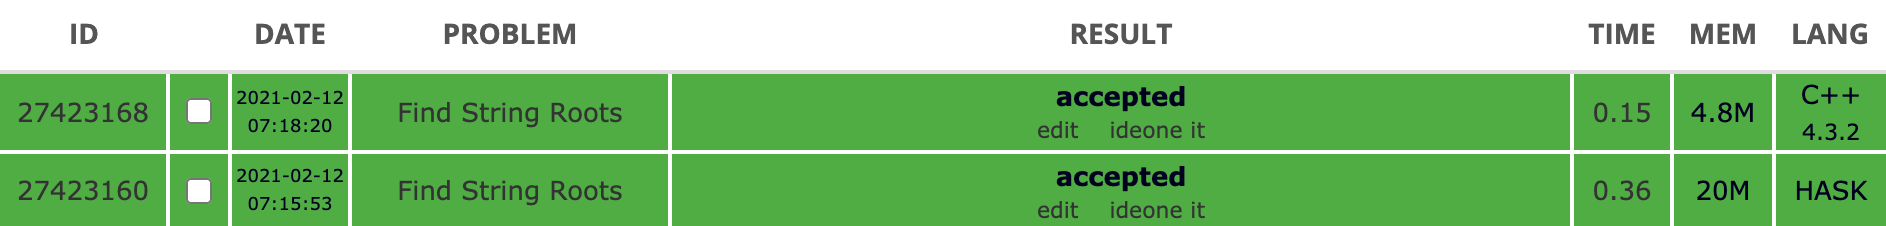
\includegraphics[width=\textwidth]{spoj/FINDSR-accepted-cpp-haskell}
\caption{El código fue aceptado por el juez en Haskell y C++}
\end{figure}

\newpage

\subsection{Ver si una cadena es una rotación cíclica de otra}
\hyperlink{cyclic_rotation}{el problema 32.4-7}
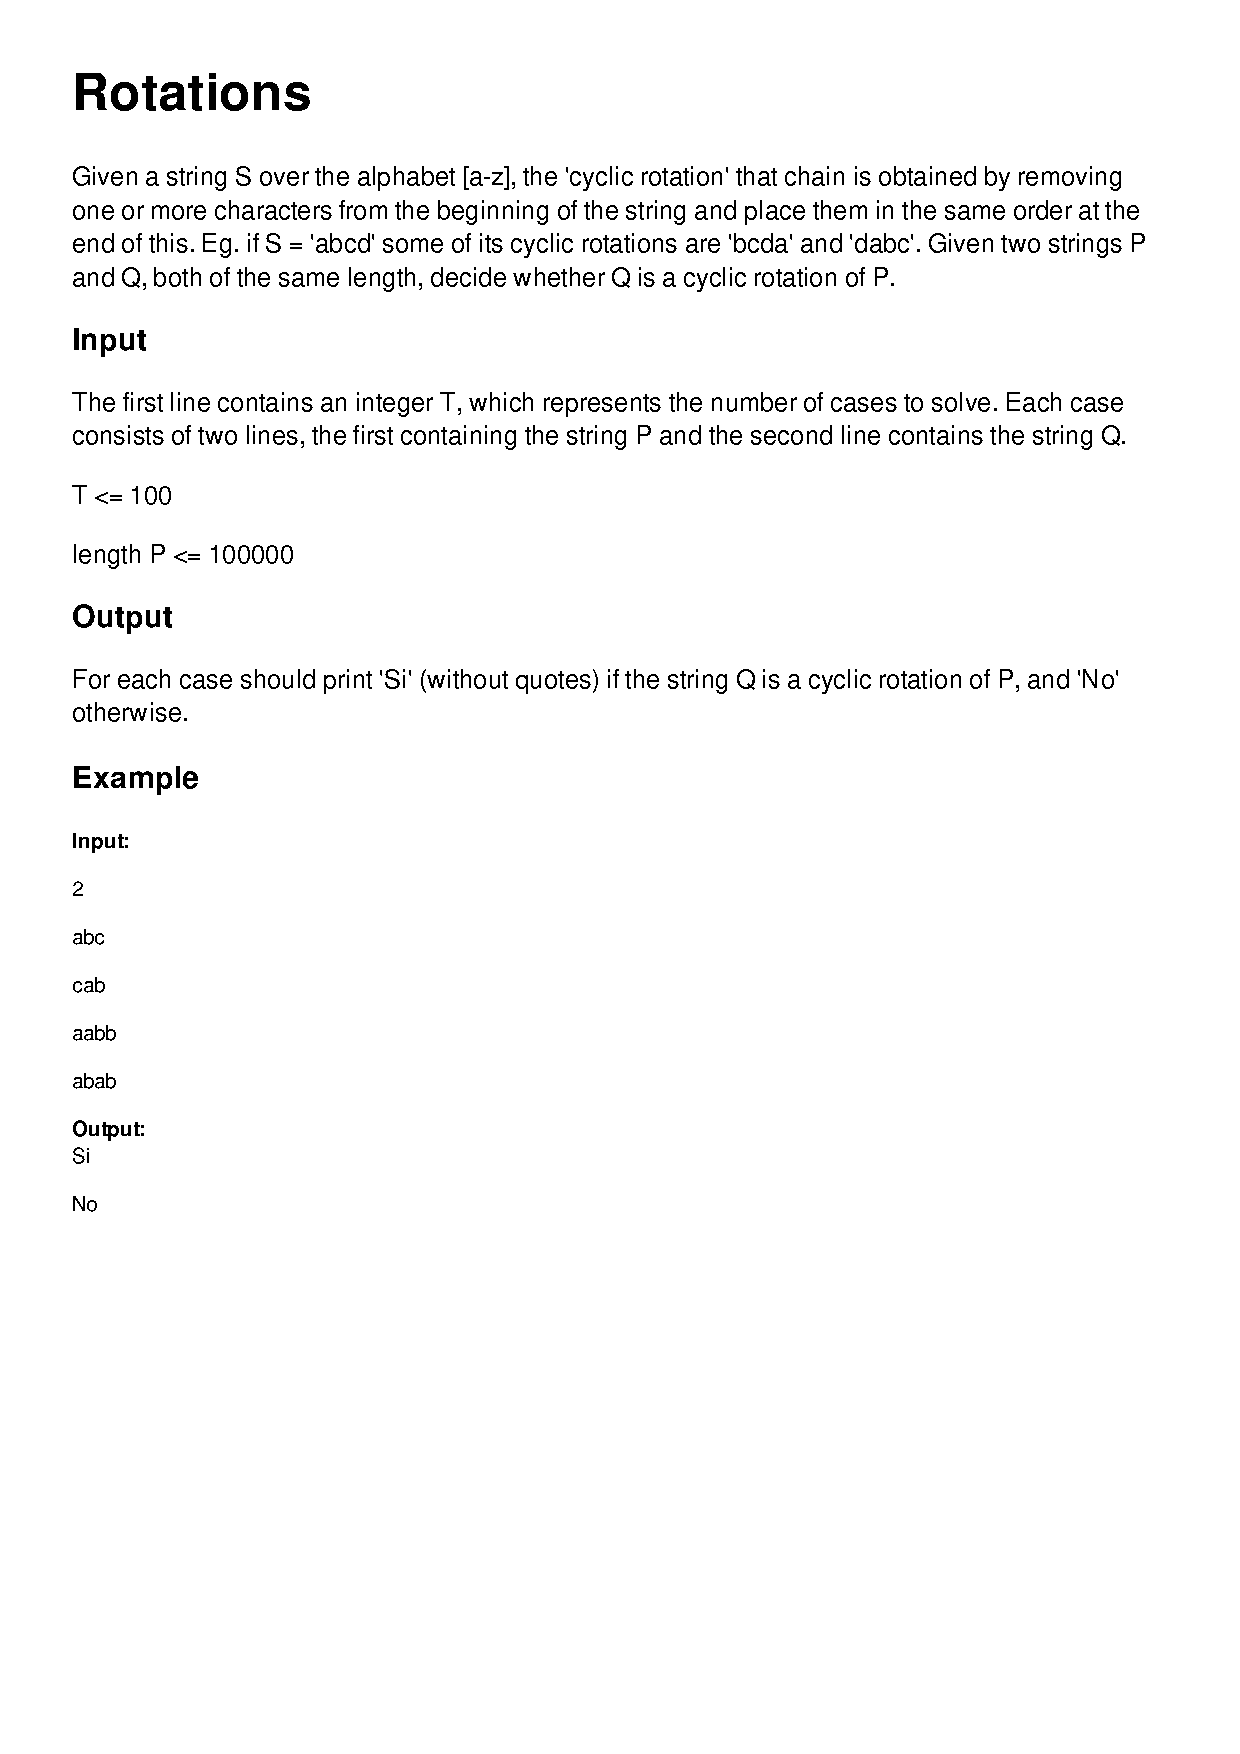
\includepdf[pages=-]{problemas/pdf/EC_WORLD.pdf}

\inputminted[linenos, frame=lines, fontsize=\footnotesize]{cpp}{problemas/cpp/EC_WORLD.cpp}
\pagebreak

\inputminted[linenos, frame=lines]{haskell}{problemas/haskell/EC_WORLD.hs}
\pagebreak

\begin{figure}[h]
\centering
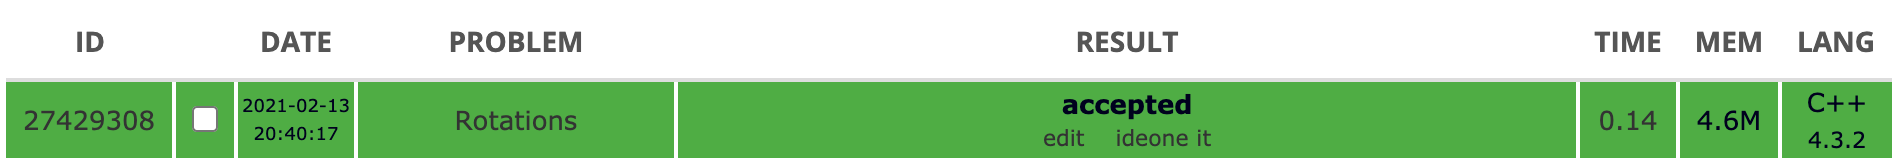
\includegraphics[width=\textwidth]{spoj/EC_WORLD-accepted-cpp}
\caption{El código fue aceptado por el juez en Haskell y C++}
\end{figure}

\subsection{Extender una cadena a un palíndromo}
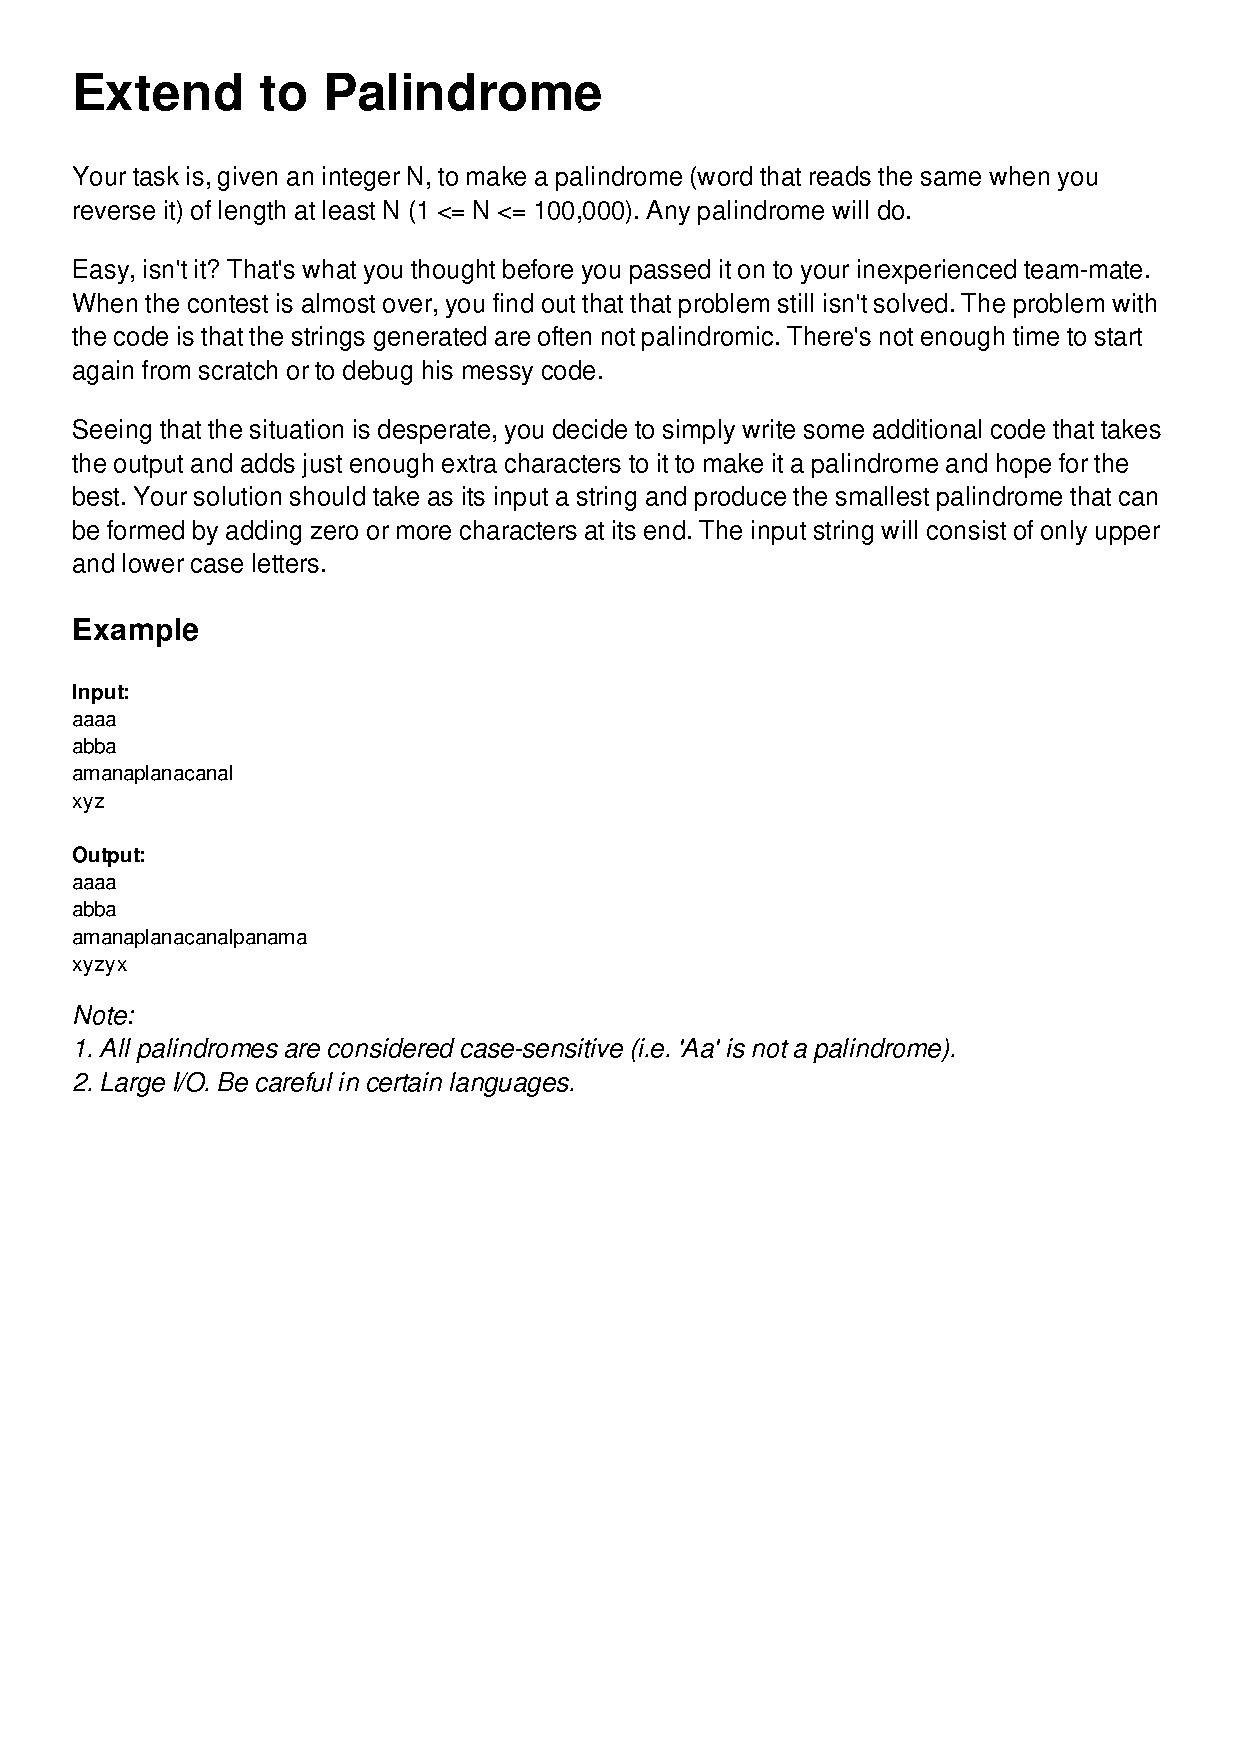
\includepdf[pages=-]{problemas/pdf/EPALIN.pdf}

\begin{figure}[h]
\centering
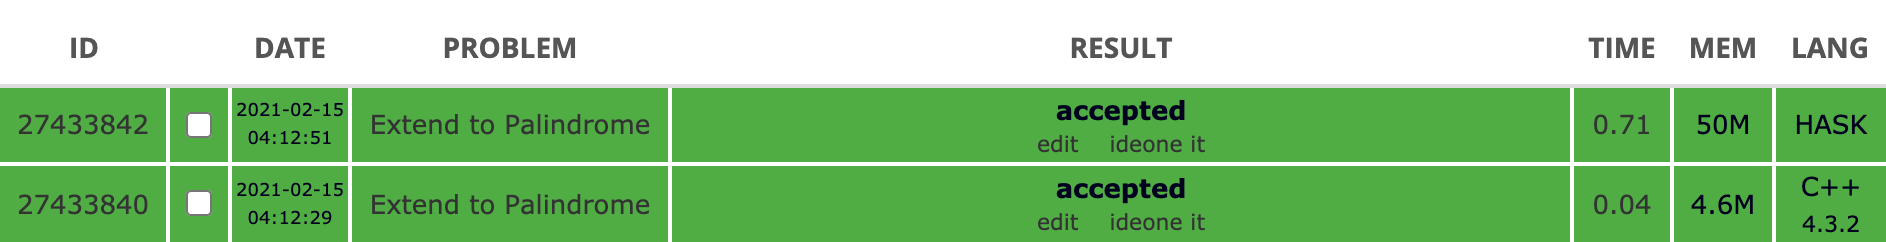
\includegraphics[width=\textwidth]{spoj/EPALIN-accepted-cpp-haskell}
\caption{El código fue aceptado por el juez en Haskell y C++}
\end{figure}

\inputminted[linenos, frame=lines]{cpp}{problemas/cpp/EPALIN.cpp}
\pagebreak

\inputminted[linenos, frame=lines]{haskell}{problemas/haskell/EPALIN.hs}
\pagebreak

\subsection{Encontrar todas las ocurrencias de un patrón en un texto}
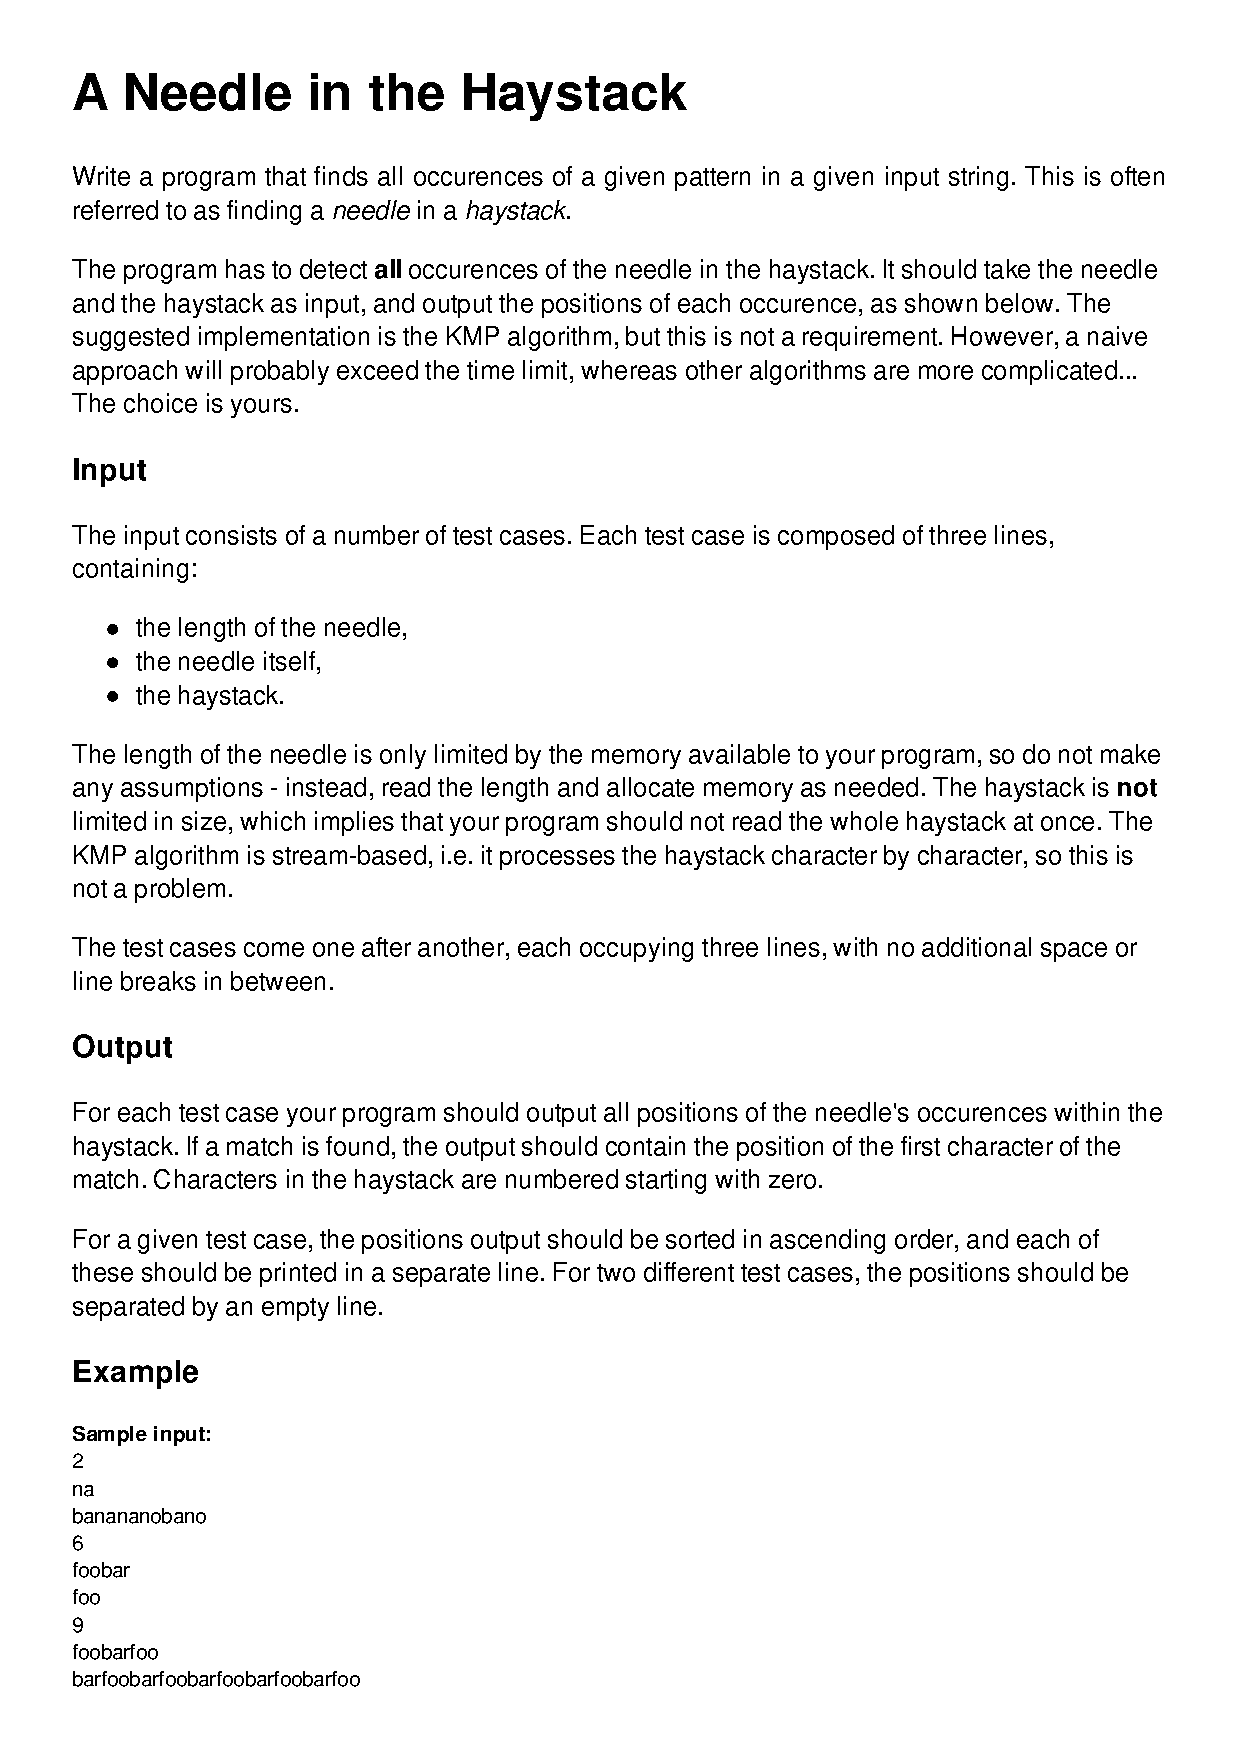
\includepdf[pages=-]{problemas/pdf/NHAY.pdf}

\inputminted[linenos, frame=lines]{cpp}{problemas/cpp/NHAY.cpp}
\pagebreak

\inputminted[linenos, frame=lines]{haskell}{problemas/haskell/NHAY.hs}
\pagebreak

\begin{figure}[h]
\centering
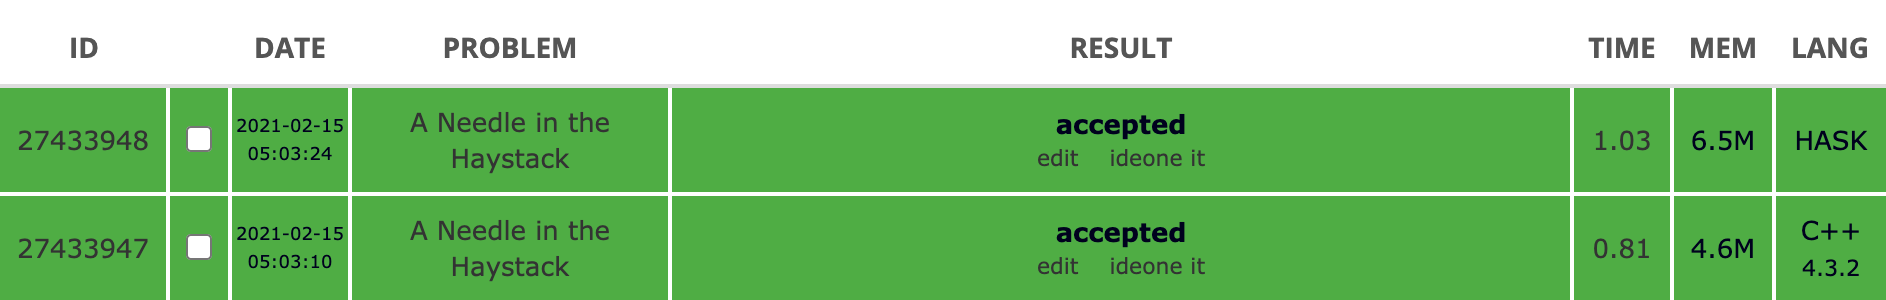
\includegraphics[width=\textwidth]{spoj/NHAY-accepted-cpp-haskell}
\caption{El código fue aceptado por el juez en Haskell y C++}
\end{figure}
% TODO: Chane y justifico esto el <$> https://ro-che.info/articles/2019-07-22-associativity-of-fmap



% TODO: poner que puedo optimizar la entrada con Data.ByteString.Char8